%%% LaTeX Template
%%% This template can be used for both articles and reports.
%%%
%%% Copyright: http://www.howtotex.com/
%%% Date: February 2011

%%% Preamble
\documentclass[paper=a4, fontsize=12pt]{scrartcl}	% Article class of KOMA-script with 11pt font and a4 format
\usepackage[margin=0.7in]{geometry}
\usepackage[english]{babel}															% English language/hyphenation
\usepackage[protrusion=true,expansion=true]{microtype}				% Better typography
\usepackage{amsmath,amsfonts,amsthm}										% Math packages
%\usepackage{color,transparent}													% If you use color and/or transparency
\usepackage[hang, small,labelfont=bf,up,textfont=it,up]{caption}	% Custom captions under/above floats
\usepackage{epstopdf}																	% Converts .eps to .pdf																		% Subfigures
\usepackage{booktabs}																	% Nicer tables
\usepackage[pdftex]{graphicx}
\usepackage{caption}
\usepackage{subcaption}
\PassOptionsToPackage{hyphens}{url}\usepackage{hyperref}

%%% Advanced verbatim environment
\usepackage{verbatim}
\usepackage{fancyvrb}
\DefineShortVerb{\|}								% delimiter to display inline verbatim text


%%% Custom sectioning (sectsty package)
\usepackage{sectsty}								% Custom sectioning (see below)
\allsectionsfont{%									% Change font of al section commands
	\usefont{OT1}{bch}{b}{n}%					% bch-b-n: CharterBT-Bold font
%	\hspace{15pt}%									% Uncomment for indentation
	}

\sectionfont{%										% Change font of \section command
	\usefont{OT1}{bch}{b}{n}%					% bch-b-n: CharterBT-Bold font
	\sectionrule{0pt}{0pt}{-5pt}{0.8pt}%	% Horizontal rule below section
	}


%%% Custom headers/footers (fancyhdr package)
\usepackage{fancyhdr}
\pagestyle{fancyplain}
\fancyhead{}														% No page header
\fancyfoot[C]{\thepage}										% Pagenumbering at center of footer
\renewcommand{\headrulewidth}{0pt}				% Remove header underlines
\renewcommand{\footrulewidth}{0pt}				% Remove footer underlines
\setlength{\headheight}{13.6pt}

%%% Equation and float numbering
\numberwithin{equation}{section}															% Equationnumbering: section.eq#
\numberwithin{figure}{section}																% Figurenumbering: section.fig#
\numberwithin{table}{section}

\usepackage[parfill]{parskip}
\usepackage{float}
\usepackage{hyperref}
\usepackage[numbers]{natbib}															% Tablenumbering: section.tab#

% use sans-serif font
\renewcommand{\familydefault}{\sfdefault}

%%% Title
\title{
	\vspace{-0.5in} 	\usefont{OT1}{bch}{b}{n}
        SEM2220: Have smartphones revolutionized the way we shop? \
}

% Authors
\author{
	\usefont{OT1}{bch}{m}{n} User ID: 110036072
	\\ \usefont{OT1}{bch}{m}{n} Aberystwyth University 
%%	\\   \texttt{slj11@aber.ac.uk}
}

\date{\today}

\begin{document}

\maketitle

\section{Introduction}
The advent of smartphones in the early 21$^{st}$ century has had a dramatic social impact on everyday life. This essay asks the question ``Have smartphones revolutionized the way we shop?''. Based on the evidence presented in this report I would be inclined to argue that they have and will continue to do so.

The number of smartphone users worldwide continues to increase worldwide with the total number of smartphone users expected to surpass the 2 billion mark by the end of 2017 \cite{emarketer2016smartphone}. As the number of smartphone users is forecasted to increase, so is the number of mobile internet users \cite{statista2016mobile}. In the UK alone Ofcom reports that 61\% of people used their mobile to access the internet last year \cite{ofcom2016facts}. Furthermore, the threshold where more users access digital content in the US via a mobile connection rather than by desktop has already been surpassed \cite{comscore2014us}. 

The mobile platform is increasingly becoming a fundamental part of peoples lives. This at least sets the foundation for significant number of people to be ready to utilise mobile commerce and it does appear to be happening. New data suggests that almost 50\% of online transactions in the UK take place on mobile \cite{econsultancy2016mobile} and mobile commerce now accounts for more than 34\% of global eCommerce \cite{criteo2015stateQ1, criteo2015stateQ4}.  


\begin{figure}[H]
    \centering
    
    \begin{subfigure}[b]{0.45\textwidth}
        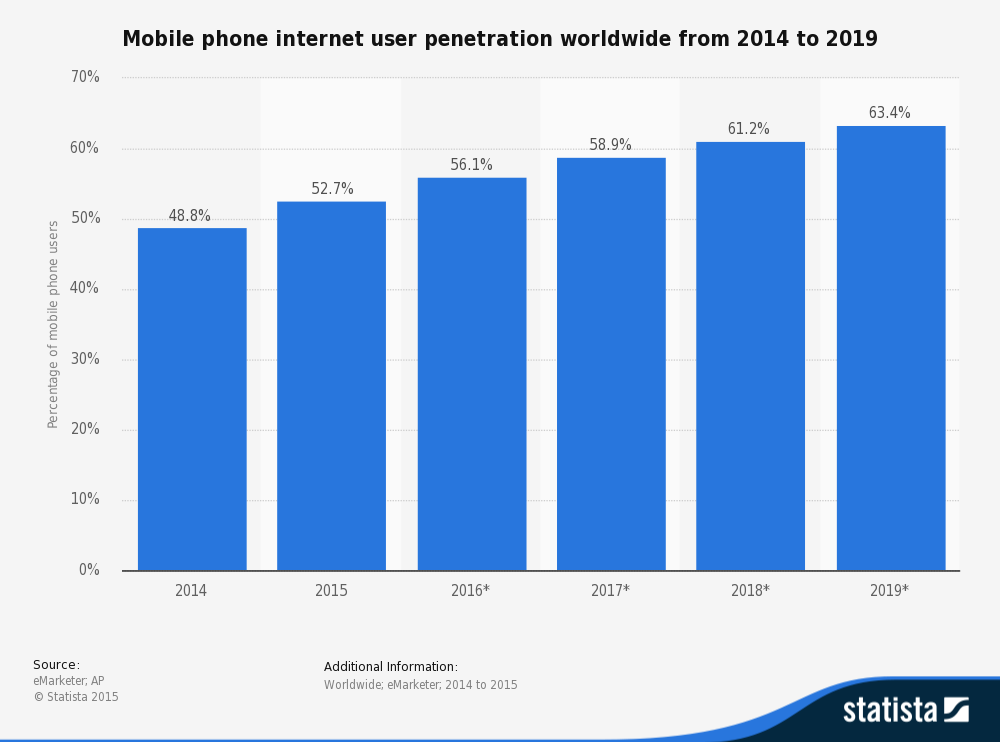
\includegraphics[width=\textwidth]{img/statistic-mobile-phone-internet-user-penetration-worldwide-2014-2019.png}
    \end{subfigure}
    ~
    \begin{subfigure}[b]{0.45\textwidth}
        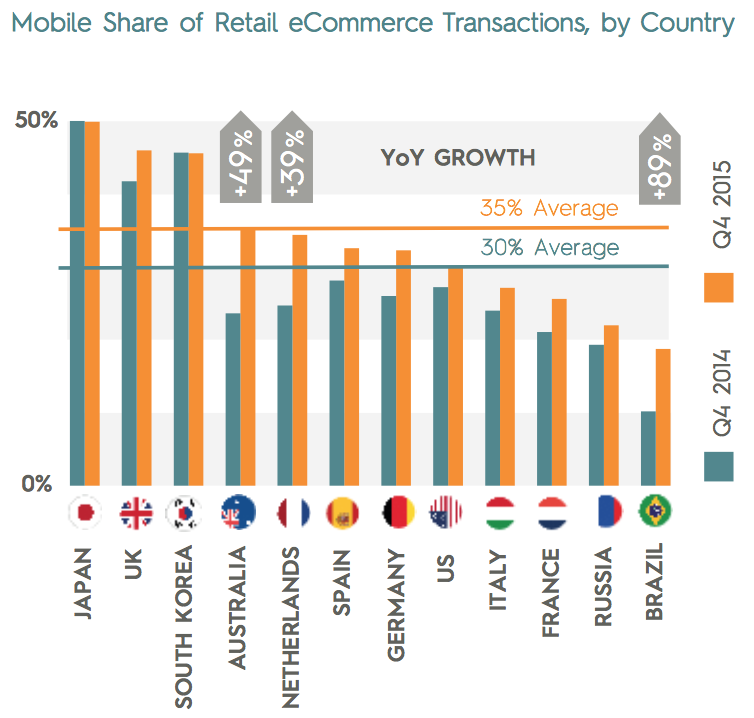
\includegraphics[width=\textwidth]{img/q4mobileshare.png}
    \end{subfigure}
    
    \caption{Left: Mobile phone internet user statistics and forecast from 2014-2019. Years marked with an asterisk are estimates. Image source: Statista \cite{statista2016mobile}. Right: Mobile retail as a share of eCommerce transactions for Q4 2015. Image source: Criteo \cite{criteo2015stateQ4}.}
    
    \label{fig:mobile-commerce}
\end{figure}

\section{Mobile Commerce Technology}

The number of ways in which consumers can perform transactions through their mobile devices has been increasing since the introduction of modern smartphones in the early years of the millennium. I would argue that this was the first boost provided by the mobile industry to commerce. The advent of the Internet had already revolutionised the way people shop. The effect that this has had on high street stores and how big online retailers (eBay, Amazon, Netflix etc.) have come to dominate the online marketplace is already evident \cite{telegraph2015internet, telegraph2015online, quartz2016online} and have forced traditional retailers to play catch-up \cite{forbes2016how}. The introduction of the mobile web has led to consumers being able to purchase goods from anywhere with an internet connection, access to which is now debatably becoming a human right \cite{larue2011report}. 

As the uptake of smartphones increased, mobile app marketplaces added new opportunities for getting your products to consumers. Beyond just the mobile web, many large businesses offer native mobile applications for there online store (e.g. Amazon, eBay) and it is now trivial to check the competitive price of goods in real time. But this concept has been taken further. Some companies, for example GBK \cite{gbk2016app}, offer apps which will give the user ``points'' collected by purchases which can lead to discounts, replacing the traditional paper discount card. Going further, apps like Groupon \cite{groupon2016app} show uses deals from numerous sites and businesses. These provide companies with a number of different ways to market to consumers and can potentially make some users more savvy as it's easier than ever to search out the best deal.

Microtransactions, transactions involving very small sums of money exchanged over the internet, have come to dominate the revenue stream from app marketplaces \cite{venture2014report}, particularly amongst the games market \cite{mashable2015micro, slice2016hardly}. I would argue that this has potentially led to an increase in expenditure within mobile marketplaces. When app marketplaces where first introduced most were separated into free and paid applications. Now with microtransactions often baked into apps many are often free to download and use with limited functionality, but cost to upgrade or add additional features.

The world is now seeing the rise of mobile point-of-sale (mPOS) technology (such as the services offered by PayPal, Square, Intuit, VeriFone etc.) for business owners and online wallets (Apple Pay, Android Pay, Samsung Pay, etc.) for customers which brings more transaction options into the world, especially when in conjunction with near field communication (NFC) technology. Adoption of these technologies beyond the boarders of the US have yet to be fully realised \cite{bbc2016google, android2016google, today2015apple}, and uptake in the US has been slow \cite{nfcworld2015trustev, pymnts2015apple} but is growing. There is also increasingly the use of paying for goods and services by scanning barcodes of QR codes at the POS or for registration for later payment. 


\begin{figure}[H]
    \centering
    
    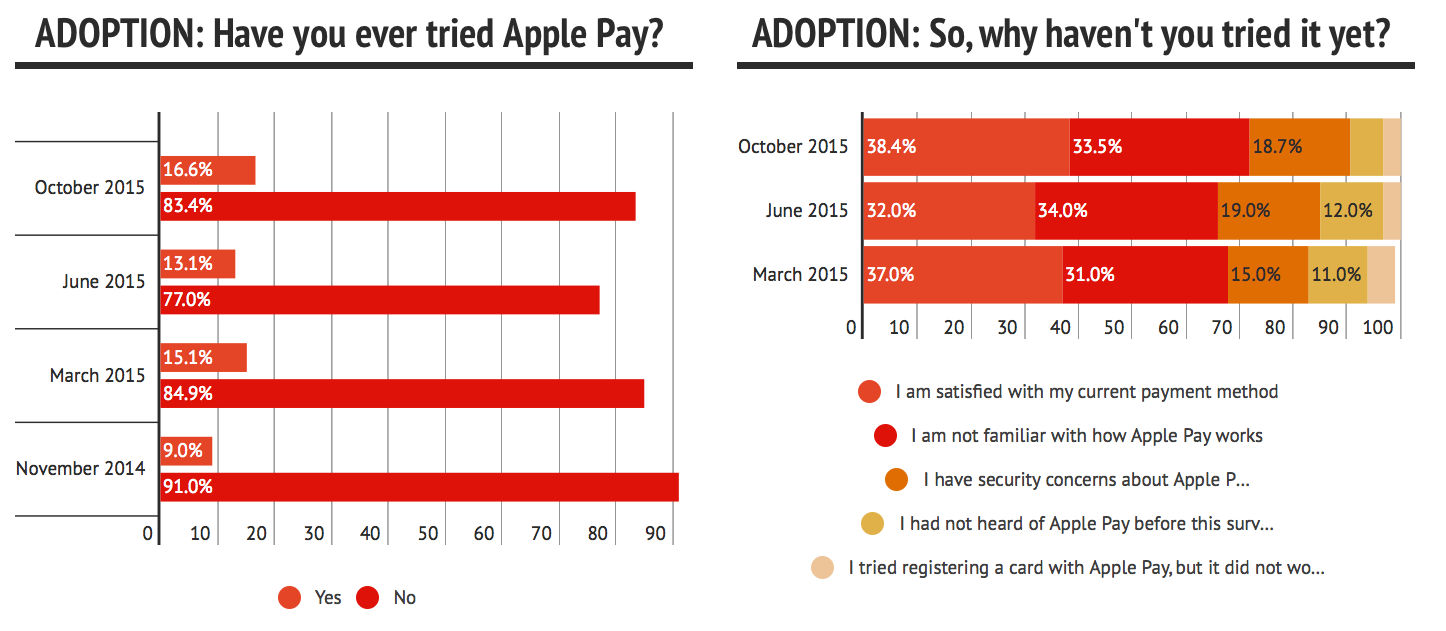
\includegraphics[width=\textwidth]{img/applepay1.png}    
    \caption{Left: Apple Pay adoption rates for select months in the past two years. Right: Reasons why consumers haven't tried Apple Pay. Image sources: PYMNTS \cite{pymnts2015apple}.}
    
    \label{fig:mobile-commerce}
\end{figure}


Could such technology lead to the rise of cashless societies? Given that credit/debit card and chip \& pin services failed to kill physical cash as a form payment this seems unlikely, at least in the immediate future. I would argue that the speed of contactless NFC payment and the ease of distribution of technology (users already have the phone) will facilitate quick adoption. Limiting factors among users are indifference, ignorance, and security. Security is likely the biggest killer as the others can possibly be mediated as awareness grows. Adoption by businesses and banks will also be a factor and the dominant players for the market have yet to be definitively established (probably Google and Apple). I'd suggest that there is also a social stigma against using cards payment for tiny sums and the slowness of chip \& pin. But micro-transactions are already a norm with mobile devices. Perhaps with the speed of NFC this stigma would disappear, and accompany reduced queuing times. 

mPOS systems have great potential for rural businesses or for business of the move. Some obvious examples might include farmers markets or couriers who have no fixed location. The other big benefit is to small business owners is no longer needing an expensive POS system. It is forecasted that there will soon be a trend towards larger businesses making use of the flexibility and cost savings offered by such systems \cite{4512015research}. However an obvious limitation to this technology is the requirement of a stable internet connection which is not always available for remote merchants.

\begin{figure}[H]
    \centering
    
    \begin{subfigure}[b]{0.7\textwidth}
        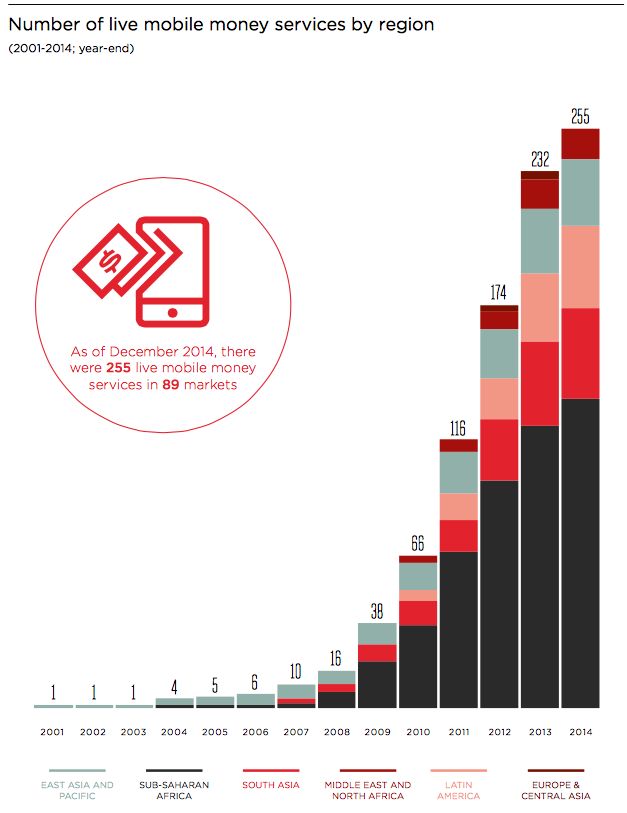
\includegraphics[width=\textwidth]{img/moneyservices.png}
    \end{subfigure}
    
    \begin{subfigure}[b]{0.7\textwidth}
        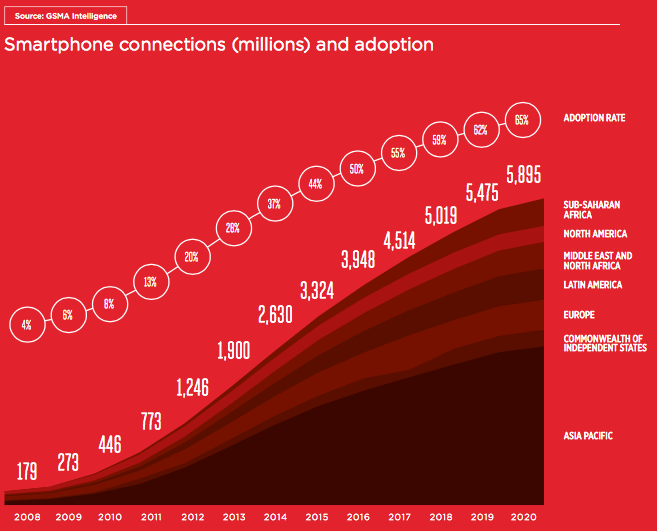
\includegraphics[width=\textwidth]{img/marketgrowth.png}
    \end{subfigure}
    
    \caption{Top: Number of live money services by region. Bottom: Smartphone adoption by region. Image sources: GSMA \cite{gsma2015mobile}.}
    
    \label{fig:mobile-commerce}
\end{figure}


Examining other demographics shows that there is a high uptake for mobile transactions in lower income economies such as Africa \cite{allafrica2016nigeria}. One particular example of note is M-Pesa \cite{mpesa2015mpesa} which has been shown to be highly successful \cite{economist2015why}. This is most likely due to a mostly cash based economy with a high level of corruption transitioning to a more secure system as the economy and infrastructure develops. Other lucrative markets up and coming markets such as BRIC countries, South America and SEA show similar promise \cite{gsma2015mobile}. These markets are likely to be highly prized and see a faster uptake because they are not yet saturated and there is no need to upgrade from existing technology.

A real sticking point in the industrialised world for the future of mobile commerce is the age gap in interest between users. A report from last year by Deloitte \cite{deloitte2015britain} showed that only ``A fifth (20\%) of 55-75 year-olds are interested in mobile payments'', compared to 34\% for people aged 18-34 in the UK. The US federal reserve \cite{federal2015consumers} showed similar figures. So a sole reliance on mobile payments would likely leave many businesses potentially missing custom.

\section{Social, Legal, and Ethical Issues}

Mobile technology has infiltrated much of our day to day lives. We are now more connected than at any other point in human history. With this technological revolution comes a social one. The pace of advancement seems to outpace the development of governing laws and ethics. Consequently there are ``grey areas'' which must be considered when adopting a new technology, both as a consumer and as a developer.

In a age where the world economy is in flux and many companies are still struggling to climb out from under the thumb of the recession it is easier than ever for consumers to make payments. Assessing whether near constant access to goods and services increase consumer spending is difficult to quantify. However I would argue that microtransactions facilitate a reduction in the awareness of how much a user is truly spending across a longer time span. The cheapness and ease of payment coupled with an addictive game or prized service can perhaps exploit users with addictive personalities. An argument could be made that it is unethical as it reinforces negative attitudes towards spending. 

Further arguments \cite{tech2015micro} have been made against ``free-to-play'' games with microtransactions because they allow players to ``pay-to-win'' offering a competitive advantage to those who can afford it. Microtransactions are perhaps worse in paid apps because you've already made a commitment to use it, but have to pay for continued use.

Another social and legal dilemma is the trust that users place in the companies and ecosystems dealing with their money. While large, trusted companies such as Google and PayPal have legal restrictions (e.g. Data Protection Act \cite{uk1998data}) to ensure that they protect consumers they are not banking institutions and large companies can go under, and they are not impervious to security vulnerabilities. 

There is also the security aspect associated with mobiles themselves. Mobiles are among the most common items stolen \cite{police2016data}. Smartphones are frequently used in public areas with high potential for personal information being observed either physically (unobscured passwords) or electronically (insecure networks). 

To take this issue further, the rise of new payment technology is likely to bring new types of fraud with it. As services like Android Pay become more popular this is likely to provide another avenue for thieves to take advantage. As slow adoption in \cite{pymnts2015apple} shows security is a concern for consumers. Card hacking devices attached to cash machines followed their rise as a payment medium. It is not unforeseeable that such exploitation will occur with NFC payment systems and not impossible that online wallet services cannot be hacked. Barcode and QR systems suffer from a verification problem. There is no way for a consumer to know that the barcode/QR code has not be replaced by a malicious agent.

One ethical issue is the use of personal data collected by apps which are used to market to the user. Often apps require permissions and privileges beyond what they really need. In the UK the  unnecessary retention of data is an infringement of the data protection act \cite{uk1998data}, but this is still a grey area if the user has explicitly given permission to the app. The ethical part of this issue can be placed with the developer. For example, does the application really need location data? Is it just for marketing purposes? It is the joint responsibility of the developer, platform, and user to ensure that the terms of permissions are clearly communicated and accepted.

\section{Conclusion}

In conclusion, I would agree with the titular question of this essay. The question is a complex socio-economic issue but I think that smartphones and mobile devices have already had an impact on how consumers pay and access goods and services. I believe that as the mobile market continues to grow and the devices and standards governing them begin to expand there will be a continued shift towards acceptance of mobile payment methods. My own opinion is that there will be a diminished, but not the eradication, of physical cash in the future. If mobile wallets or some similar technology are accepted by consumers and business alike then it is not hard to imagine chip and pin systems heading the same way as cheques. 

The biggest point the in preceding paragraph is the ``if'' in the final sentence. Smartphones have unquestionably become integrated into our society, but there is still a question over whether they will become an permenatly accepted medium for managing commerce. There are still many legal and security concerns surrounding widespread adoption, as with all new types of technology. But I believe that the consumer desire is there and that is the major driver for smartphones to continue to revolutionise how we shop.

\bibliographystyle{unsrtnat}
\bibliography{references}
\end{document}
